\section{Antecedentes y Estado del Arte}

\subsection{Satélites Definidos por Software}

Resulta revelador observar cómo la noción de software-defined networking, exitosa en entornos terrestres, ha migrado al dominio espacial con consecuencias profundas. Los satélites definidos por software (SDS) han pasado de ser una idea prometedora a una realidad operativa en menos de una década. 

Jiang et al. \cite{Jiang2023} ofrecen una de las revisiones más completas disponibles, donde describen la evolución desde los primeros prototipos hasta las arquitecturas actuales que permiten reconfigurar en órbita no solo la capa de enlace sino también aspectos del procesamiento de payloads. Entre las técnicas clave destacan el uso de hipervisores ligeros, virtualización de funciones de red (NFV) adaptadas al espacio y herramientas de simulación que permiten validar configuraciones antes de su despliegue orbital. 

Sin embargo, tras años de observar estos desarrollos, cabe matizar que la flexibilidad conseguida sigue siendo predominantemente reactiva. La mayoría de las plataformas SDS actuales dependen de comandos terrenales para cambiar su comportamiento, limitando su capacidad de respuesta inmediata ante eventos impredecibles. Esta brecha entre potencial teórico y capacidad real constituye precisamente uno de los motores principales del presente trabajo.

\begin{table}[h]
\centering
\caption{Comparativa de arquitecturas SDS representativas}
\label{tab:arquitecturas_sds}
\begin{tabular}{lccc}
\hline
\textbf{Arquitectura} & \textbf{Flexibilidad} & \textbf{Procesamiento Cognitivo} & \textbf{Año Ref.} \\
\hline
Tradicional (bent-pipe) & Baja & Nula & -- \\
SDS Clásico & Media & Limitada & 2020-2023 \\
SDS Cognitivo (propuesto) & Alta & Alta & Este trabajo \\
\hline
\end{tabular}
\end{table}

\subsection{Procesamiento de Señales en SDR}

Uno de los desafíos persistentes al analizar plataformas SDR en el contexto satelital radica en la tensión entre reprogramabilidad y rendimiento en tiempo real. Aunque los radios definidos por software han liberado a los ingenieros de la rigidez del hardware dedicado, tienden a operar con algoritmos de procesamiento fijos que resultan vulnerables ante las dinámicas propias del canal espacial.

Particularmente llamativo es el hecho de que técnicas clásicas de filtrado, sincronización y demodulación, altamente eficientes en condiciones controladas, degradan con rapidez bajo efectos combinados de Doppler elevado, fading severo y niveles variables de ruido. En muchos casos estudiados, los sistemas SDR convencionales requieren intervención humana o configuraciones conservadoras que sacrifican eficiencia espectral en favor de robustez. 

Doha et al. \cite{Doha2026} documentan esta evolución, mostrando cómo el procesamiento de señales ha transitado gradualmente desde métodos puramente matemáticos hacia enfoques híbridos que incorporan elementos adaptativos. No obstante, la mayor parte de estas soluciones permanecen en la categoría de ``adaptativas'' más que verdaderamente cognitivas.

\subsection{IA en Comunicaciones Satelitales}

Lejos de ser un asunto resuelto, la integración de inteligencia artificial en comunicaciones satelitales revela tanto promesas como limitaciones importantes. Doha et al. \cite{Doha2026} presentan una taxonomía detallada que permite apreciar el recorrido desde los primeros intentos basados en machine learning clásico hasta las aproximaciones más recientes basadas en deep learning y reinforcement learning.

Aunque los modelos de deep learning han demostrado excelente capacidad para tareas como clasificación automática de modulación (AMC) y estimación de parámetros, su aplicación directa en entornos orbitales enfrenta obstáculos serios de computación y consumo energético. Resulta especialmente interesante contrastar estos enfoques con soluciones más tradicionales.

de Senneville et al. \cite{deSenneville2025} ofrecen un ejemplo práctico valioso al aplicar machine learning para detección y mitigación de interferencias en señales de telecomunicaciones espaciales utilizando SDR. Sus resultados destacan ventajas claras en escenarios under-determined, donde los métodos convencionales tienden a fallar. Sin embargo, también ponen de manifiesto limitaciones en generalización cuando las condiciones del canal se alejan significativamente de los datos de entrenamiento.

\begin{figure}[h]
\centering
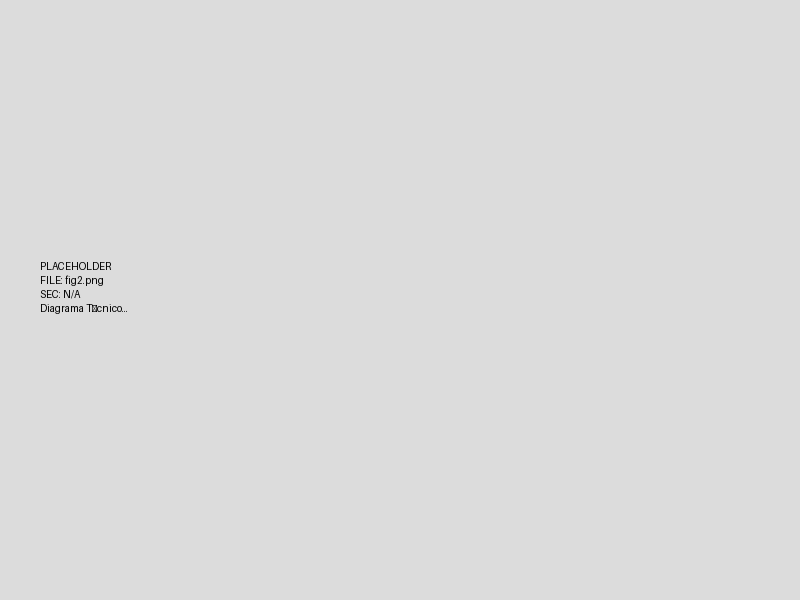
\includegraphics[width=\linewidth]{fig2.png}
\caption{Taxonomía de técnicas de IA aplicadas a procesamiento de señales en SDR satelitales.}
\label{fig:taxonomia_ia_sdr}
\end{figure}

En síntesis, el estado del arte revela un progreso sostenido en componentes aislados, pero persiste una brecha notable en la integración holística de capacidades cognitivas dentro de plataformas SDS con restricciones reales de vuelo. Esta observación motiva directamente la arquitectura propuesta en la siguiente sección.